
\documentclass[a4paper]{IEEEtran}

% Ein paar hilfreiche Pakete
\usepackage[utf8]{inputenc}
\usepackage[T1]{fontenc}
\usepackage{ngerman}
\usepackage{graphicx}
\usepackage{amsmath}
\usepackage{amssymb}
\usepackage{mathtools}
\usepackage{subcaption}
\usepackage{hyperref}


\usepackage{url}
\usepackage{breakurl}
\usepackage[breaklinks]{hyperref}

\def\UrlBreaks{\do\/\do-}

% Nummeriere Formel nur, wenn sie auch referenziert wird
\mathtoolsset{showonlyrefs}

% Header
\markboth{Seminar SS 16: Anthropomatik praktisch erfahren}{Seminar SS 16: Anthropomatik praktisch erfahren}

% Hier den Titel des eigenen Seminars eintragen
\title{Kinect Punktwolken in die Unreal Engine importieren}

% Hier deinen eigenen Namen
\author{Marius Wodtke}


\begin{document}

% Erzeugt die Überschrift
\maketitle

% Zusammenfassung
\begin{abstract}
	Die Immersion ist ein wichtiger Aspekt für den Reiz von virtuellen Welten. 
	Aktuelle VR Systeme haben große Fortschritte bei der Anzeige der Welt selbst gemacht, der eigentliche Nutzer ist in ihr aber oft ein Fremdkörper.
	Die mangelnde Fähigkeit den Nutzer insgesamt zu erfassen führt dazu, dass er zu einem Augenpaar und einem Paar Händen wird. 
	Technologien wie die Kinect erlauben es jedoch den Nutzer als Ganzes zu erfassen, sie soll genutzt werden, damit der Nutzer sich selbst und andere in der virtuellen Welt sehen kann.
	Diese Arbeit soll in Vorbereitung darauf einen Prototyp erstellen, der die Bilder einer Kinect in die Unreal Engine importiert und sie dort zu einer Punktwolke verarbeiten und anzeigen soll.
	Er ist für eine Kinect voll funktionsfähig, für die Verarbeitung mehrerer aber nicht leistungsfähig genug.
\end{abstract}

% Erster Abschnitt
\section{Einleitung}
	Technische Entwicklungen wie {\textit{head-mounted displays}} haben die Erfahrung der Telepräsenz in den letzten Jahren deutlich verbessert. 
	Aber um sich an einem entfernten beziehungsweise virtuellen Ort wirklich anwesend zu fühlen reicht es nicht die Bewegung des Nutzers korrekt zu übersetzen. 
	Zusätzlich muss die Welt und die Personen in ihr passend dargestellt werden. \\
	Aktuelle VR-Brillen wie die \textit{HTC VIVE} zeichnen nur die Position der Brille und der Controller auf, Systeme die den gesammten Körper aufzeichnen benötigen typischerweise sehr viel Vorbereitung, wie etwa das Anbringen von Reflektoren am Körper des Nutzers. 
	Optische Systeme zur Erkennung, wie etwa die Microsoft Kinect, sind nach einer einmaligen Kalibrierung deutlich schneller einsatzbereit. 
	Dabei ist es möglich aus den aufgenommenen Bildern wieder eine dreidimensionale Punktwolke erzeugt werden und so den Nutzer in der virtuellen Welt darzustellen. \\
	Werden die Brille und die Punktwolke der Kinect korrekt aufeinander abgestimmt sollte der Nutzer danach in der Lage sein sich selbst in der virtuellen Welt zu sehen.\\
	
\section{Aufbau der Arbeit}
	Zunächst wird die zu bearbeitende Aufgabe definiert, anschließend wird die verwendete Hardware, eine Microsoft Kinect v2.0, vorgestellt. Dann werden zwei Ansätze zur Integration in die Unreal Engine diskutiert: Erst das Kinect 4 Windows Plugin und danach der PCViewer, der für die Bearbeitung der Aufgabenstellung verwendet wird. Nun wird die Projektion der Kamerabilder in den dreidimensionalen Raum und das Zeichnen der Punktwolke erörtert. Abschließend wird ein Fazit gezogen.


\section{Aufgabenstellung}
	Aufgabe soll es sein, die von der Kinect ausgegebenen Streams in die frei verfügbare Unreal Engine zu importieren, dort soll aus dem Tiefenbild und dem Farbbild eine dreidimensionale Punktwolke erzeugt werden. 
	Dabei beschränkt sich diese Arbeit auf eine Kinect. \\
	Dies dient als Vorbereitung für die in der Einleitung motivierte Übertragung des menschlichen Körpers in die virtuelle Welt. \\

\begin{figure}[!h]
    	\centering
		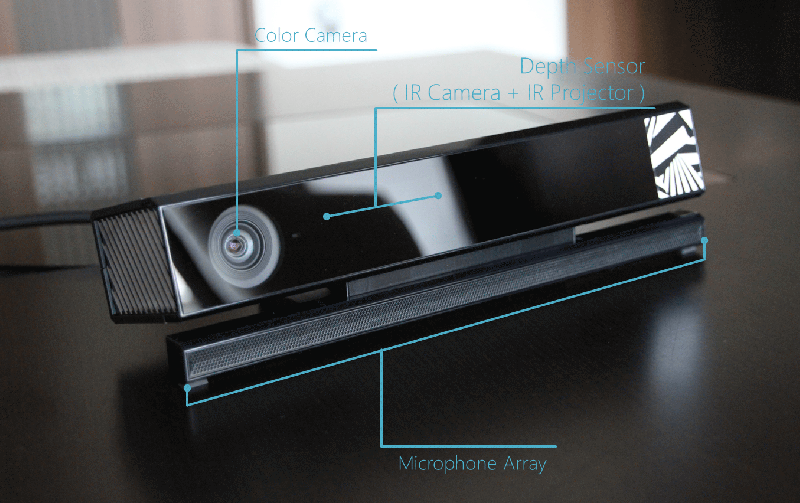
\includegraphics[width=0.5\textwidth]{img/Kinectv2}
	    \caption{Microsoft Kinect v2.0, Farbkamera und Tiefensensor können zur Erzeugung einer Punktwolke verwendet werden. {\cite{kinectpic}}}
    	\label{Kinectv2}
	\end{figure}
	
\section{Microsoft Kinect}
	Die Kinect wurde ursprünglich von Microsoft für die Xbox 360 entwickelt bietet eine Farbkamera, einen Infrarotprojektor, eine Infrarotkamera und mehrere Mikrofone, sie wurde Ende 2010 veröffentlicht (siehe Abb. \ref{Kinectv2}). \\
	Gut ein Jahr später veröffentlichte Microsoft ein \textit{Software Development Kit}, zusammen mit einem Adapter kann man unter Windows Applikationen entwickeln, die die Kinect nutzen.
	Als Einschränkung gilt aber jederzeit, dass der Treiber nur eine Kinect pro Rechner verarbeitet: "{}Kinect for Windows supports one sensor, which is called the default sensor"{} {\cite{kinectone}}.\\
	Wichtig für diese Arbeit ist, dass Infrarotprojektor und Infrarotkamera zusammen einen Tiefensensor bilden. 
	Kombiniert man diesen Tiefensensor und Farbkamera kann man eine Punktwolke erzeugen, dazu müssen die Pixel des Kamerabildes entlang der Tiefeninformation in den dreidimensionalen Raum projeziert werden. 
	Die dazugehörige Software ermöglicht noch viele andere Interpretationsarten der gelieferten Bilder, zum Beispiel kann sie ein Knochenmodell von Personen vor der Kamera berechnen, diese können dann in Avatare umgesetzt werden, die die Bewegungen der Personen kopieren.
	Für diese Arbeit wird die Kinect v2.0 verwendet. \\[0.5cm]
	
	
	
\section{Kinect 4 Windows v2.0 Plugin}
	Das Kinect 4 Windows v2.0 Plugin ermöglicht es die verschiedenen Input Streams der Kinect in die Unreal Engine zu importieren. Das Plugin setzt dabei bereits eine funktionierende Kinect voraus, es müssen zunächst die {\textit{Kinect Runtime}} {\cite{kinectruntime}} und das {\textit{Kinect SDK}} {\cite{kinectsdk}} installiert werden. \\
	Anschließend sollte die Kinect getestet werden, dazu kann der {\textit{PCViewer}} des ISAS verwendet werden. 
	Zunächst wird der Server ({\textit{PCViewer}}) und anschließend der Client ({\textit{Node}}) gestartet, nun sollte die Kinect im Menu des Servers erscheinen und es können die {\textit{Color-}} und {\textit{Depth-Streams}} aktiviert werden. 
	Sieht man nun eine Punktwolke, die dem Blickwinkel der Kamera entspricht, funktioniert alles wie vorgesehen.\\
	

\section{Projektmappe erstellen}
	Zunächst klont man das GitHub Projekt KinectDemoRoom {\cite{k4w}}. 
	Nach einem Rechtsklick auf die .uprojekt Datei muss zunächst die Version 4.9 der Unreal Engine ausgewählt werden, danach können im selben Menu die Projektdateien erstellt und eigentlich auch kompilliert werden, letzteres schlägt aber fehl und es muss ein Kompilerfehler von Hand behoben werden. \\
	Dazu muss muss das Projekt in Visual Studio geöffnet werden (.sln Datei) und  im {\textit{KinectV2Module}} für die {\textit{PrivateDependencyModuleNames}} und {\textit{PublicDependencyModuleNames}} der Eintrag {\textit{"{}UnrealEd"{}}} hinzugefügt werden, weiteres zu dem Problem ist in den Issues {\cite{k4wissues}} zu finden.\\
	
	\begin{figure}[!h]
    	\centering
		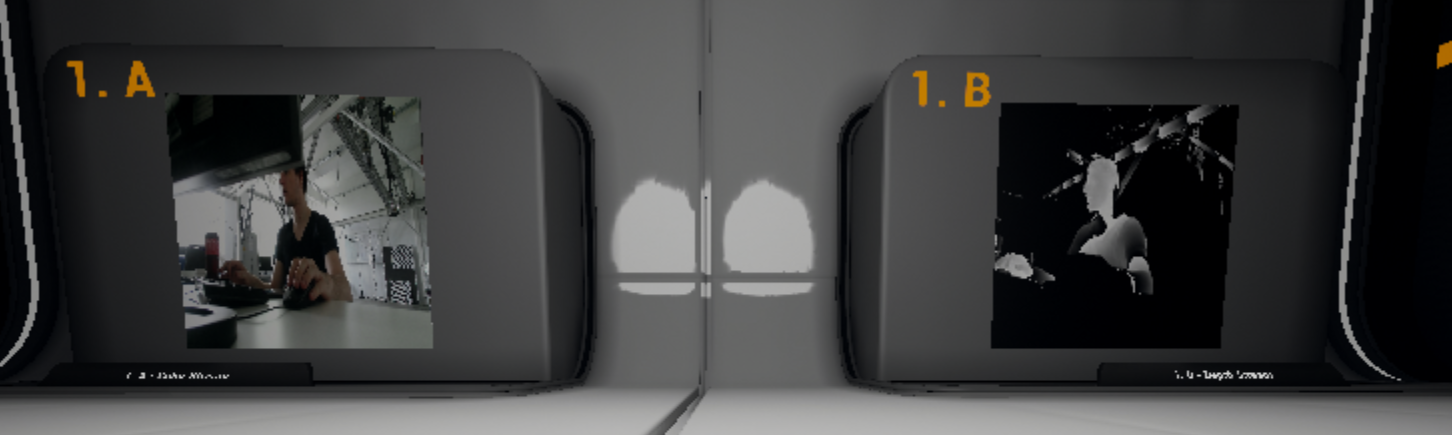
\includegraphics[width=0.5\textwidth]{img/Kinect4Windows}
	    \caption{Die Kinect 4 Windows Demo Umgebung, es werden Farb- und Tiefenbild visualisiert.}
    	\label{Kinect4Windows}
	\end{figure}


\section{Blueprint}
	Nachdem die Projektmappe erfolgreich erstellt wurde sollte sich die .uproject Datei öffnen lassen und der Unreal Editor startet.
	Zu Spielbeginn muss zunächst die Kinect gestartet werden, wichtig ist auch sie bei Spielende wieder abzuschalten, sonst läuft sie die ganze Zeit. 
	Die Grundfunktionalität des Plugins beinhaltet das Auslesen der Input Streams wie Farbe, Tiefe und Infrarot (Abb. \ref{Kinect4Windows}).
	Eine Implementierung für die Berechnung und Darstellung einer Punktwolke ist noch nicht integriert.
	Um die Input Streams zu erhalten können {\textit{Event Dispatcher}} angelegt werden, an die passende Events gebunden werden. 
	Diese liefern bei jedem ankommenden Bild der Kinect ein Ereignis und das Bild als Textur zurück, diese lässt sich gut auf Flächen projezieren, die Projektion auf einzelne Pixel gestaltet sich schwieriger. \\
	Um das Farbbild hierfür nutzbar zu machen muss die Textur in ein Array mit {\textit{LinearColor}} Werten umgewandelt werden, die Werte des Arrays können dann einzeln ausgelesen und als Pixelfarben gesetzt werden (siehe Abb. \ref{2DColor}). 
	Eine Funktion zur Umwandlung stellt der Unreal Editor nicht zur Verfügung, sie muss als C++ Funktion hinzugefügt werden. 
	Ähnliches gilt für die Tiefeninformation, die ebenfalls als Textur kodiert werden. 
	Sind die Farb- und Tiefeninformationen eines Frames in Arrays verpackt kann man beginnen die Punktwolke zu erzeugen.\\
	Bei diesem Plugin besteht aber immer das Problem, dass das Plugin direkt mit dem Treiber zusammen arbeitet, es kann also immer nur eine Kinect ausgelesen werden. 
	Dies ist im Zusammenhang der Motivation nicht sinnvoll, da mindestens zwei Kameras auf gegenüberliegenden Seiten verwendet werden müssen um ein vollständiges dreidimensionales Modell eines Körpers zu erhalten.
	Das Plugin wurde daraufhin zugunsten des PCViewers verworfen.\\

	\begin{figure}[!h]
    	\centering
		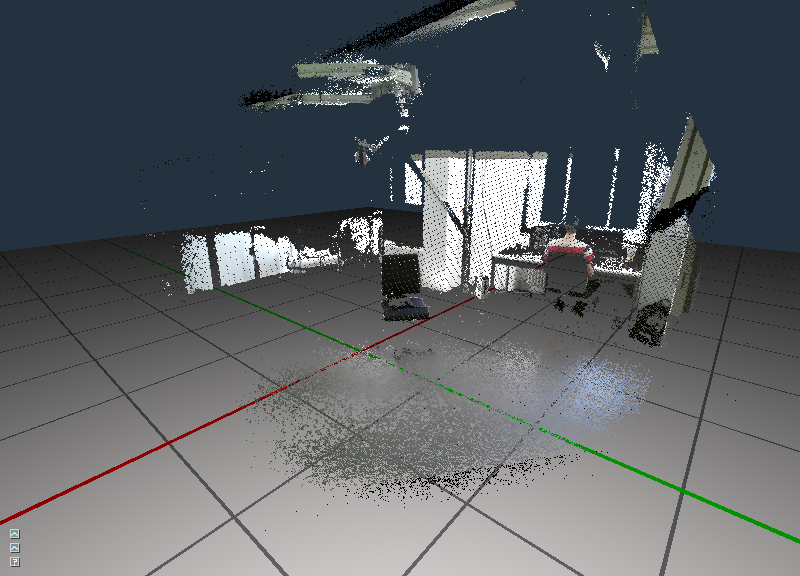
\includegraphics[width=0.5\textwidth]{img/CloudPCViewer}
	    \caption{Die Ansicht einer Punktwolke im Point Cloud Viewer.}
    	\label{CloudPCViewer}
	\end{figure}
	


\section{PCViewer}
	Der {\textit{PCViewer}} ist eine Applikation des ISAS, sie spaltet sich in einen Client und einen Server. 
	Ein Client kann die Bilder der Kinect auslesen und diese über das Netzwerk an den Server verschicken. 
	Der Server empfängt die Daten und kann diese auch für andere Anwendungen bereitstellen.\\
	Mit diesem System können mehrere Kinects verarbeitet werden, dabei muss natürlich nach wie vor jede Kinect an einen eigenen Rechner angeschlossen werden, aber nun besteht die Möglichkeit, alle auf einem zentralen Rechner zu nutzen.
	Der PCViewer kann außerdem in der graphischen Oberfläche bereits Punktwolken anzeigen, dies wird als Referenz für die korrekte Darstellung in der Unreal Engine dienen (vgl. Abb. \ref{CloudPCViewer} und Abb. \ref{Cloud}). \\
	Das {\textit{e-installation}} Projekt benutzt den PCViewer bereits in Kombination mit der Unreal Engine, allerdings um das verwendete {\textit{head-mounted display}} auszulesen. 
	Deshalb sind die Funktionen zum Auslesen einer Kinect noch nicht implementiert, sie müssen genauso wie die Berechnung der Punktwolke hinzugefügt werden. \\[0.5cm]
	
		\begin{figure}[!h]
    	\centering
		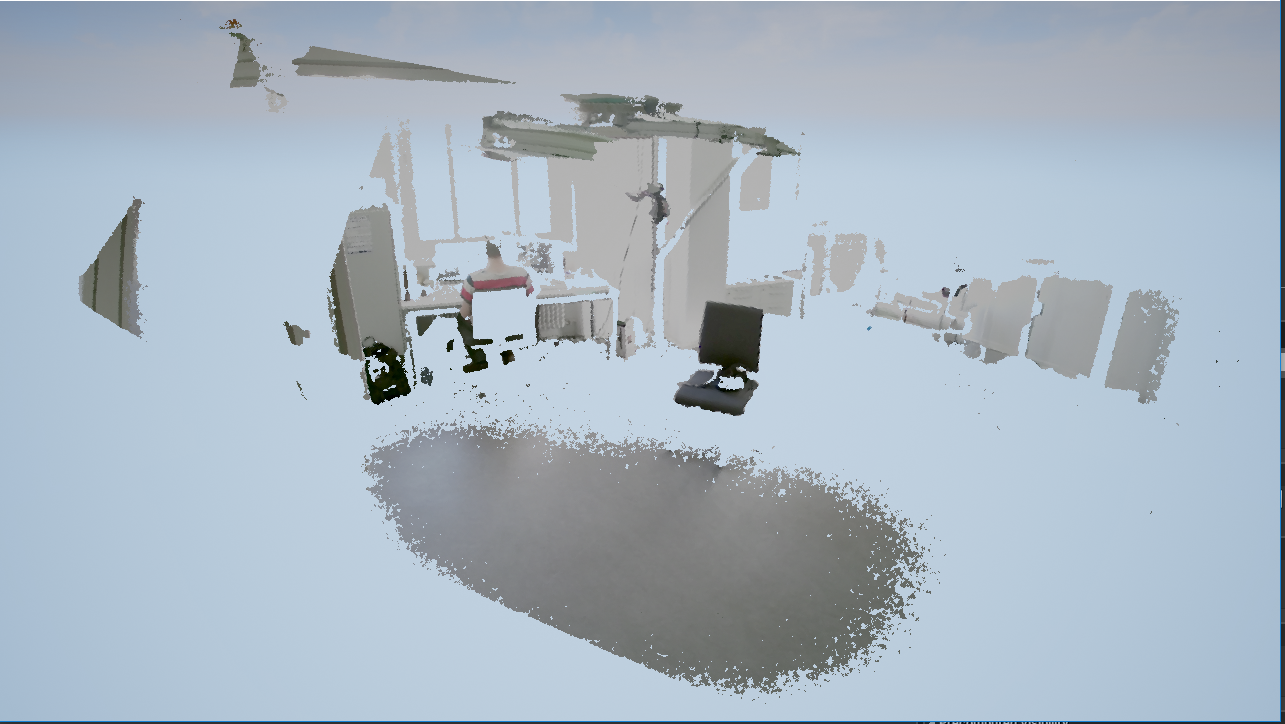
\includegraphics[width=0.5\textwidth]{img/Cloud}
	    \caption{Das Ergebnis der Integration einer Punktwolke in die Unreal Engine.}
    	\label{Cloud}
	\end{figure} 

\section{Funktionen}
	Wie bereits im vorigen Abschnitt beschrieben fehlen der Unreal Engine Schnittstelle des PCViewers noch einige Funktionen zum Auslesen der Kinect Streams. 
	Das eigentliche Auslesen ist dabei trivial, weil man nur den PCViewer anweisen muss das jeweilige Bild in einem gegebenen Puffer zur Verfügung zu stellen. 
	Um die Farb- und Tiefenbilder dann aber für die Unreal Engine nutzbar zu machen, müssen sie in TArrays gespeichert werden und die Datentypen in solche umgewandelt werden, die die Unreal Engine verarbeiten kann. \\
	So muss zum Beispiel ein Puffer mit einem Farbbild durchlaufen werden und immer drei uint8 (RGB-)Werte zum einer Linear Color komponiert und dem TArray angehängt werden.
	Die für die Transformation in den dreidimensionalen wichtige intrinsche und extrinsische Kameramatrix wird auf die selbe Weise ausgelesen und in eine ITransform umgewandelt. \\
	Die Berechnung der Position der Punktwolke mit dem Tiefenbild und den Kameramatrizen wird im folgenden Abschnitt {\ref{projektion}} beschrieben, anschließend beschäftigt sich Abschnitt {\ref{zeichnen}} mit der Darstellung der Punktwolke. \\
	Alle implementierten Funktionen sind in Abbildung \ref{AllFunctionsBP} aufgeführt.\\[0.5cm]
	
	\begin{figure}[!h]
    	\centering
		\includegraphics[width=0.5\textwidth]{img/Functions}
	    \caption{Die für den Prototypen entwickelten Funktionen. {\textit{Get Extrinsic}} wurde bereits vom {\textit{e-installation}} Projekt implementiert.}
    	\label{AllFunctionsBP}
	\end{figure}


\section{Projektion in den dreidimensionalen Raum}
\label{projektion}
	Während die Kameras der Kinect einen konischen Bereich aus der Welt aufzeichnen, bilden sie diesen natürlich auf ein zweidimensionales Bild ab. 
	Dabei wird jeder dreidimensionale Punkt $[y_1,y_2,y_3]^T$ mit der intrinsischen Kamera-Matrix \\ [1cm]

\begin{center}
$I = \begin{bmatrix}
f_u & 0 & c_u  \\
0 & f_v & c_v  \\
0 & 0 & 1  
\end{bmatrix}$\\[1cm]
\end{center}

	in ein einen zweidimensionalen Pixel und eine Tiefe $[u,v,1]^T \times \gamma$ transformiert. 
	Dabei bezeichnen $f_u$ und $f_v$ die Fokuslänge und $c_u$ und $c_v$ den Hauptpunkt. 
	Ein Punkt des Tiefenbildes berechnet sich also aus \\[1cm]

\begin{center}
$\begin{bmatrix}
u \\
v \\
1
\end{bmatrix}
\times
\gamma
= \begin{bmatrix}
f_u & 0 & c_u  \\
0 & f_v & c_v  \\
0 & 0 & 1  
\end{bmatrix}
\times
\begin{bmatrix}
y_1 \\
y_2 \\
y_3
\end{bmatrix}$\\[1cm]
\end{center}

	Für die Projektion in den dreidimensionalen Raum der virtuellen Realität muss mit $[y_1',y_2',y_3']^T = I^{-1} \times [u,v,1]^T \times \gamma$ aus jedem Punkt des Tiefenbildes und dem Inversen der intrinsischen Kamera-Matrix ein Punkt im dreidimensionalen Raum berechnet werden \cite{TEO}.
	Die Formel lautet \\[1cm]

\begin{center}
$\begin{bmatrix}
y'_1 \\
y'_2 \\
y'_3
\end{bmatrix}
= \begin{bmatrix}
\frac{u - c_u}{f_u} \\
\frac{v - c_v}{f_v}  \\
1  
\end{bmatrix}
\times
\gamma$.\\[1cm]
\end{center}

	Der berechnete Punkt ist relativ zum Ursprung. 
	Wenn nur eine Kinect benutzt wird ist dies kein Problem, man verschiebt einfach den Ursprung in der Unreal Engine um die Punktwolke an die gewüschnte Position zu bekommen. 
	Sollen aber mehrere Kinects zum Einsatz kommen müssen die Kameras in Position und Rotation koordiniert werden, dazu kann die extrinsische Matrix $E$ definiert werden. \\[1cm]

\begin{center}
$\begin{bmatrix}
y_1 \\
y_2 \\
y_3
\end{bmatrix}
= E
\times
\begin{bmatrix}
y'_1 \\
y'_2 \\
y'_3
\end{bmatrix}$\\[1cm]
\end{center}

\begin{figure}[!h]
    	\centering
		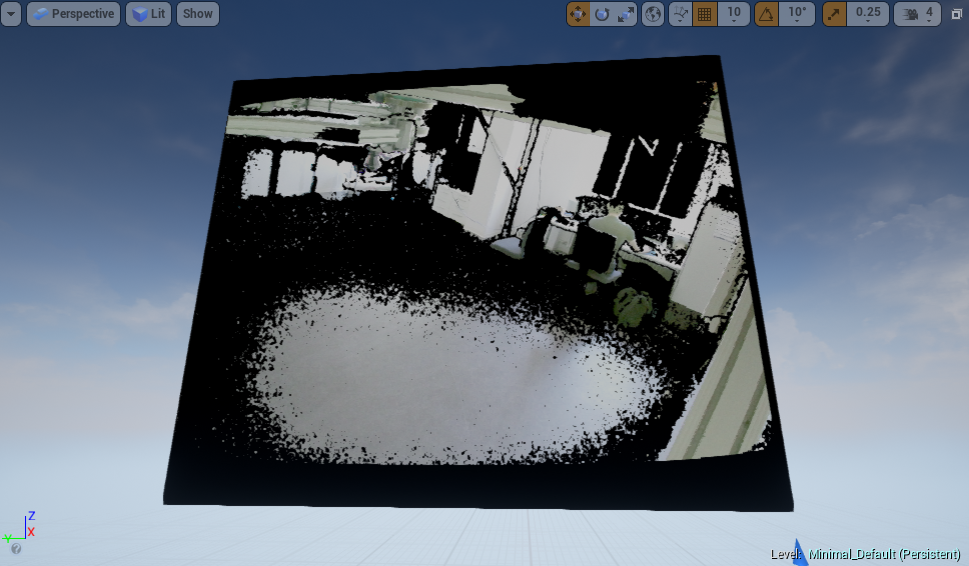
\includegraphics[width=0.5\textwidth]{img/2DColor}
	    \caption{Die Anzeige des Farbildes mit der {\textit{Draw Debug Point}} Funktion. Für zweidimensionale Anzeigen sollten Texturen verwendet werden, dies ist deutlich effizienter.}
    	\label{2DColor}
	\end{figure} 
	


\section{Zeichenfunktionen}
\label{zeichnen}
	Nach der Berechnung der Positionen muss nur noch ein Punkt an jede davon gezeichnet werden. 
	Die Unreal Engine bietet mit {\textit{Draw Debug Point}} eine einfache Methode um farbige Punkte an festgelegte dreidimensionale Positionen zu zeichnen, leider ist sie eher für sporadische und nicht für massenhafte Verwendung ausgelegt. \\
	Auf dem Referenzrechner werden nur wenige Millionen Punkte pro Sekunde gezeichnet. 
	Eine Kinect kann allerdings 30 Bilder pro Sekunde liefern, das ergibt bei 217.088 Pixeln pro Bild (512x424) mehr als 6,5 Millionen Pixel pro Sekunde. \\
	Einige davon können eingespart werden. 
	Pixel, deren Tiefe nicht richtig erkannt wurde werden nicht aus der Kamera herausprojeziert, sie müssen nicht gezeichnet werden. 
	Hinzu kommen Pixel, bei denen die Farbe nicht erkannt wurde, sie säumen zumeist die korrekt erkannten Bereiche und erzeugen einen schwarzen Rand. 
	Auch sie werden übersprungen um Zeichenoperationen zu sparen. 
	Dies hebt die anzeigbare Bildrate auf eine einigermaßen flüssige Darstellung - aber nur für eine Kinect. \\
	Um mehrere Kinect gleichzeitig zu verarbeiten braucht es deshalb eine andere Zeichenfunktion.
	Dies wurde bereits im Unreal Forum diskutiert {\cite{lidar}}.
	Die Verwendung von soliden Objekten wie etwa Würfeln hat zwar den Vorteil, dass sie nicht immer wieder neu erzeugt werden müssen, man kann sie einfach versetzen und die Oberfläche neu färben. 
	Allerdings besitzen dreidimensionale Objekte im Gegensatz zu Punkten mehrere Oberflächen die gerendert werden müssen, dies frisst die Vorteile wieder auf.\\
	{\textit{Particles}} in einem {\textit{Particle System}} können sehr performant erzeugt werden. 
	Sie sollten sich auch für die Darstellung mehrerer Kinect eignen, allerdings werden die Particles kollektiv kontrolliert und nicht einzeln gesetzt. 
	Um sie also zu nutzen müsste man sich eine Methode überlegen die Particles mit kollektiver Kontrolle die Punktwolke bilden zu lassen und sie in den richtigen Farben darzustellen. \\[0.5cm]
	
	


\section{Fazit}
	Der für diese Ausarbeitung angefertigte Prototyp Anwendung zeigt exemplarisch, dass es möglich ist Kinect Streams in die Unreal Engine zu importieren und zu verarbeiten.
	Dabei sollten sie in der C++ Anbindung der UE verarbeitet werden, denn die Verarbeitung ist sehr aufwändig und die Bilder in Blueprints zu verarbeiten führt zu einem Flaschenhals.\\
	Der Prototyp kann eine Kinect von einem anderen Rechner zu importieren, mehrere gleichzeitig zu verarbeiten dürfte jedoch wegen dem Aufwand der verwendeten {\textit{Draw Debug Point}} Funktion problematisch werden. 
	Die in der Aufgabenstellung bezeichnete Aufgabe wurde also erfüllt, bezogen auf die Motivation sind aber noch Anpassungen des Prototyps notwendig.
	Um der flüssigen Anzeige eines Körpers in der VR zu genügen muss dieser nämlich von mehreren Kinect von verschiedenen Seiten aufgenommen - und verarbeitet - werden. 
	Die resultierende Größe der Punktwolke ist für diesen Prototyp zu viel, er könnte sie nur wenige Male pro Sekunde zeichnen. 
	Hohe Bildraten sind in der virtuellen Realität aber wichtig, damit der Nutzer sich in ihr präsent fühlt und nicht an der Simulatorkrankheit leidet. \\[0.5cm]
	

	


% Literaturverzeichnis in Literatur.bib
% (z.B. per Hand oder mit Zotero, Jabref, etc. editieren) 
\Urlmuskip=0mu plus 1mu\relax
\bibliographystyle{plain}
\bibliography{Literatur}
\end{document}

